\documentclass[useAMS,usenatbib]{mn2e}
\usepackage{graphicx}

%\usepackage{tikz}
\newcommand{\aap}{Astron. Astrophys.}
\newcommand{\aj}{Astron. J.}
\newcommand{\ao}{Appl. Opt.}
\newcommand{\apj}{Astrophys. J.}
\newcommand{\apjl}{Astrophys. J. Lett.}
\newcommand{\apjs}{Astrophys. J. Suppl.}
\newcommand{\mnras}{Mon. Not. Roy. Ast. Soc.}
\newcommand{\nat}{Nature}
\newcommand{\pasa}{Publ. Ast. Soc. Aust.}
\newcommand{\pasp}{Publ. Ast. Soc. Pac.}
\newcommand{\prl}{Phys. Rev. Lett.}
\newcommand{\prd}{Phys. Rev. D}
\newcommand{\msun}{\mathrm{M}_\odot}

\title[2MPZ and LIGO]{Using the 2-MASS Photometric Redshift Survey to optimize LIGO Follow-Up Observations}
\author[Antolini \& Heyl]{Elisa Antolini$^{1}$, Jeremy S. Heyl$\thanks{Email:
    heyl@phas.ubc.ca; Canada Research Chair}^{2}$ \\
  $^{1}$Dipartimento di Fisica e Geologia, Universit\`a degli Studi di Perugia, I-06123 Perugia, Italia \\
  $^{2}$Department of Physics and Astronomy, University of British
  Columbia, 6224 Agricultural Road, Vancouver, BC V6T 1Z1, Canada\\
}
\begin{document}
\date{Accepted ---. Received ---; in original form ---}

\pagerange{\pageref{firstpage}--\pageref{lastpage}} \pubyear{2015}

\maketitle

\label{firstpage}

\begin{abstract}
  The initial discovery of LIGO on 14 September 2015 was the in-spiral
  merger and ring-down of the black hole binary at a distance of about
  500~Mpc or a redshift of about 0.1.  The search for electromagnetic
  counterparts for the in-spiral of binary black holes is impeded by
  poor initial source localizations and a lack of a compelling model
  for the counterpart; therefore, rapid electromagnetic follow-up is
  required to understand the astrophysical context of these sources.
  Because astrophysical sources of gravitational radiation are likely
  to reside in galaxies, it would make sense to search first in
  regions where the LIGO-Virgo probability is large and where the
  density of galaxies is large as well.  Under the Bayesian prior
  assumption that the probability of a gravitational-wave event from a
  given region of space is proportional to the density of galaxies
  within the probed volume, one can calculate an improved localization
  of the position of the source simply by multiplying the LIGO-Virgo
  skymap by the density of galaxies in the range of redshifts.  We
  propose using the 2-MASS Photometric Redshift Galaxy Catalogue for
  this purpose and demonstrate that using it can dramtically reduce
  the search region for electromagnetic counterparts.
\end{abstract}

\section{Introduction}

LIGO has recently begun to detect gravitational wave events from the
local Universe \citep{PhysRevLett.116.061102}.  During these initial
years of gravitational astronomy, the localization of the candidate
events on the sky is poor with the ninety-percent confidence regions
covering hundreds or even thousands of square degrees.  Finding an
electromagnetic counterpart to these candidate graviational-wave
events will be crucial to understanding what produces them,
interpretation of the signal and to provide tests of general
relativity.  The ideas of how the the electromagnetic counterparts
would appear are varied and uncertain. There has been substantial
speculation on the electromagnetic transients associated with the
mergers of binaries that include a neutron star
\citep[e.g.][]{2016PhRvD..93b4011E,2016arXiv160107711K,2016arXiv160100017D,2015arXiv151205435F,2015ApJ...814L..20M,2015PhRvD..92d4028K,2015arXiv150807939S,2015arXiv150807911S}
However,the first discovered gravitational wave event (GW150914)
appears to be the merger of binary black holes, so the appearance and
duration of the electromagnetic counterparts are especially uncertain
with only a few models
\citep[e.g.][]{2015PhRvL.115n1102G,2015MNRAS.452.3419M,2016MNRAS.457..939C,2016ApJ...817..183Y}
Consequently, rapid electromagnetic follow-up of a large portion of
the probable region would increase the chance of success in finding a
counterpart.  Over the large search regions and over the span of days
or weeks, many electromagnetic transients typically occur, and with
the wide variety of models it will be difficult to associate
unambigously a particular electromagnetic event with a candidate
gravitational-wave event.

The purpose of this paper is to present a strategy to alleviate both
of these issues; that is, to reduce both the search region and the
time required to plan and begin observations.  We follow the spirit of
\citet{2015arXiv150803608G} to develop a galaxy catalogue to guide the
observational plan.  However, our goal here is to develop a nearly
complete catalogue at the expense of having less accurate estimates of
the redshifts of the galaxies within the catalogue.  The accuracy of
the galaxy distances needs to be only as good as the distance estmates
of the gravitational-wave events.  Additionally we will outline a
straightforward and rapid technique to generate a nearly optimal
observing plan to follow up the events rapidly (i.e. within a few
seconds of the trigger). 

\section{Bayesian Approach to Follow-Up}

Because we will be interested in the rapid follow-up of candidate
gravitational-wave events, we will focussed on the rapid Bayesian
reconsruction outlined by \citet{2015arXiv150803634S}, BAYESTAR.  At
the most basic level, BAYESTAR yields a probability map on the sky in
the form of a HEALPpix map \citep{2005ApJ...622..759G} where each
pixel contains the probability $P(d|m)$ that a particular model
(i.e. position on the sky) will yield the data (i.e. the observed
strains on the LIGO and Virgo interferometers).  To plan an observing
strategy one would like the probability of a particular model
(i.e. position on the sky) given the data.  We have from Bayes's
theorem
\begin{equation}
  P(\mathrm{position}|\mathrm{data}) = \frac{P(\mathrm{position})
    P(\mathrm{data}|\mathrm{position})}{P(\mathrm{data})}.
  \label{eq:1}
\end{equation}
If we make the additional mild assumption that gravitational-waves
originate from nearby galaxies, the probability of a given position on
the sky naturally is proportional to the density (or perhaps the
luminosity density) of galaxies in that direction integrated over
distance range determined from the modelling of the gravitational
waveform.  Of course, these distance estimates will usually have large
uncertainities so the distance range over which to integrate the
galaxy density distribution will also be large, so highly accurate
redshift information is not needed to construct
$P(\mathrm{position})$.

Furthermore, because we will ultimately be interested in which fields
to observe (not which particular galaxies), accurate positions are not
required in the construction of $P(\mathrm{position})$. It is natural
to sample $P(\mathrm{position})$ also as a HEALPix grid with each pixel
covering about the same solid angle as the field of view of the
telescope of interest or the BAYESTAR map (a HEALPix $\mathtt{NSIDE}=512$ or
about 50 square arcminutes per pixel), so positions no more accurate
than arcminutes are required.  The key to generate the observing plan
rapidly is to calculate the required galaxy density maps beforehand in
principle at the desired resolution (this optimization only speeds the
process up slightly) for the distance ranges of interest.  With the
arrival of an alert, all that is required is to calculate
Eq.~(\ref{eq:1}) using the HEALPix maps, resample to the scale of the
telescope, renormalize the probability, sort the pixels from most
likely to least and output the positions to cover a given amount of
cumulative probability (this entire process takes typically less than
one second).

\section{Galaxy Catalogues}

To gain a picture of the local Universe, our focus will be the
completness of the data rather than the accuracy of the distances and
positions.  \citet{2015arXiv150803608G} combine several redshift
surveys
\citep[e.g.][]{2002MNRAS.336..907N,2003MNRAS.344..307L,2005MNRAS.360...81D,
  2012ApJS..199...26H} that cover a large portion of the sky, but at
various depths and attempt to increasing the completeness of the
sample by using only the galaxies near the upper-end of the luminosity
function ({\em i.e.}  $L\sim L_*$) and ; the discovery that binary
black holes with large masses (!)  dominate the initial detections
indicates that focussing the search on massive galaxies might not be
the best strategy.  After all such large black holes have not been
found so far in our approximately $L_*$-galaxy, the Milky Way, or our
neighbour, Andromeda.  In fact theoretical arguments indicate that the
production of such massive black holes results from the evolution of
massive stars in low metallicity galaxies
\citep{2016ApJ...818L..22A,2016arXiv160203790E} which are typically
small in the local Universe \citep[e.g.][]{1997MNRAS.285..613H}. Our
goal is to have a nearly complete survey that attempts to be unbiased
with respect to the mass of the galaxy.

We follow in spirit the work of \citet{2004PASA...21..396J} who used
The Two Micron All Sky Survey extended source catalogue \citep[2MASS
  XSC,][]{2000AJ....119.2498J,2006AJ....131.1163S}, and the assuption
that all galaxies have the `same $K_s-$band luminosity of around $L_*$
to estimate distances to each galaxy and create sky maps of the local
Universe.  A substantial fraction of 2MASS has measured redshifts
\citep[e.g][]{2012ApJS..199...26H}.  \citet{2014ApJS..210....9B}
combined the photometric data from 2MASS XSC with additional
photometry the mid-infrared from WISE \citep{2010AJ....140.1868W} and
the optical from SuperCOSMOS
\citep{2001MNRAS.326.1315H,2001MNRAS.326.1295H,2001MNRAS.326.1279H}.
Using this multiband photometry, they trained neural networks using
measured spectroscopic redshifts from SDSS
\citep{2012ApJS..203...21A,2014ApJS..211...17A}, 2dF
\citep{2001MNRAS.328.1039C,2003astro.ph..6581C}, 6dF
\citep{2004MNRAS.355..747J,2009MNRAS.399..683J} and other catalogues
to determine photometric redshifts.  They also extend the photometric
redshift catalogue beyond the 2MASS XSC building a three-dimensional
map of the sky out to a redshift of nearly 0.2 well into the realm of
the first gravitational wave event.  The 2MASS Photometric Redshift
(2MPZ) catalogue contains over one million galaxies with a median
redshift of 0.1 with a typical scatter between the
photometric and spectroscopic redshifts (where both are known) of
$\sigma_z = 0.015$.

Except for the most local sources, the estimate distances from the
gravitational wave data itself have comparable errors to this, so this
catalogue is sufficiently accurate to calculate the surface density of
galaxies with the expected redshift range of a particular
gravitational-wave detection.  Furthermore, for the nearest sources,
there are nearly uniform all-sky redshift surveys which would be more
appropriate for this task
\citep[e.g][]{2000MNRAS.317...55S,2012ApJS..199...26H}.  Of course, all
of the techniques outlined here can be applied to these more nearby
catalogues to produce sky maps of even more nearby galaxies.  Here we
will focus on galaxies with photometric redshifts between 0.01 and 0.1
from the 2MPZ catalogue as depicted in Fig.~\ref{fig:galmap}.  For closer
galaxies the redshift error is significant, and the outer end of the
range is both the median redshift of the catalogue and the typical
distances of the binary-black-hole sources.
\begin{figure}
  \includegraphics[width=\columnwidth]{2MPZgz_001_01_smoothed}
  \caption{The relative surface density of galaxies in the 2-MASS Photometric Redshift Survey with photometric redshifts between 0.01 and 0.1, smoothed with a Gaussian of 0.6 degrees (0.01 radian).}
  \label{fig:galmap}
\end{figure}

To produce this map we divided the sky into 3,145,728 regions (each of
about 45 square arcminutes, four ACS fields) using a HEALPix
\citep{2005ApJ...622..759G} tesselation with $\mathtt{NSIDE}=512$.
Each cell of the map simply contains the number of galaxies in the
2MPZ catalogue within the range of photometric redshift that lie
within that portion of sky.  We have subsequently smoothed the map
with a Gaussian with $\sigma=0.01$ radian.  Typically no HEALPix pixel
contains more than one galaxy from the catalogue.  After smoothing we
notice the large-scale structure even when we have averaged over
distance.  This demonstrates the potential optimization in the
observing strategy by observing fields with nearby galaxies. Depending
on whether one believes that the sources are associated with the
visible portion of galaxies or may travel some distance from the
galaxy itself before the gravitational-wave event, one would use
either the raw galaxy counts or the smoothed map.

Furthermore, our choice of weighting the fields simply by the number
of galaxies within each field is perhaps the most simple one.  Given
the type of event, one could use a map that gives small,
low-metallicity galaxies more weight or weigh the galaxies by their
mass or luminosity.  Of course, all of these possibilities would be
informed by one's prior knownledge of the source inspired by
theoretical models and the hints from the waveform itself and give a
better estimate of $P(\mathrm{position})$.  The key is to calculate these
maps beforehand.

\begin{figure}
  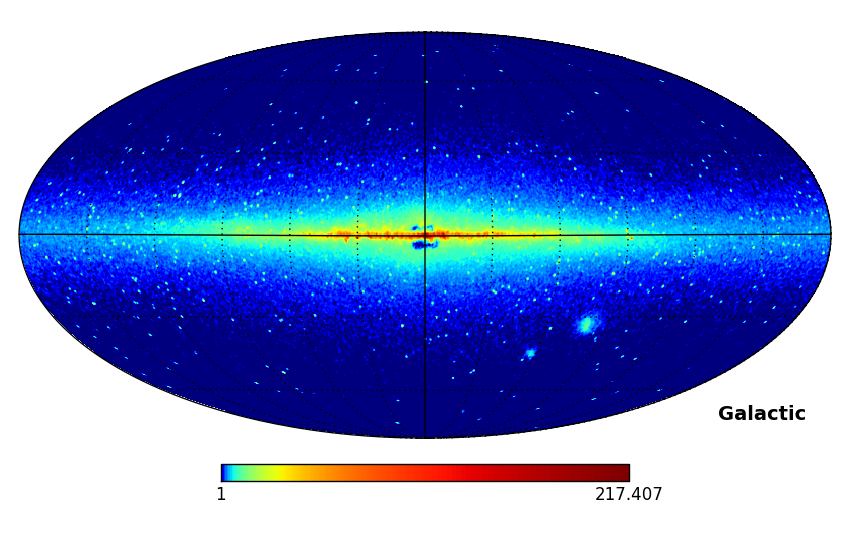
\includegraphics[width=\columnwidth]{2mass_density}
  \caption{The relative surface brightness of stars in the 2-MASS
    Photometric Catalogue \citep{2006AJ....131.1163S} smoothed with a Gaussian of 0.03 degrees (0.005 radian).}
  \label{fig:starmap}
\end{figure}
There is a further structure apparent in the map, and this is of
course the zone of avoidance imposed by the disk and bulge of our
Galaxy. Depending on the nature of the follow-up
({\em e.g.} gamma-ray and radio) observations it may make
sense to include regions along the Galactic plane where one thinks
nearby galaxies should be. One can attempt to probe the zone of avoidance
\citep[e.g][]{2000AJ....120..298J} and future 21-cm surveys like CHIME
\citep{2014era..conf10102V} will also probe the large-scale structure
beyond the Galactic plane.   However, the existing galaxy density map
as depicted in Fig.~\ref{fig:galmap} can yield an estimate of the
structure obscured by the Galaxy.  The technique that we will use in
similar to that used by \citet{2008StMet...5..289A} to inpaint the CMB
anisotropies across the Galactic plane.

Here we will determine the region masked by the Galaxy by finding the
region in which the density of galaxies is either less than one tenth
of the mean (from Fig.~\ref{fig:galmap}) or in which the density of
stars (from Fig.~\ref{fig:starmap}) is greater than a threshold that
accounts for the masking of the background galaxies due to the Large
Magellanic Cloud, a feature that is apparent in both figures.  Both of
these masks are nearly the same, so we combine them as depicted in the
upper panel of Fig.~\ref{fig:infilling}.  This region is much narrower
than the infilled region of the CMB in \citet{2008StMet...5..289A},
and furthermore the observed structures the galaxy map are typically
longer than the width of the mask, so we can reliably estimate the
hidden structures.  In spite of these differences the basic strategy
is similar.  We assume that the underlying galaxy map (behind the
Galaxy) is isotropic; therefore, it is natural to represent it as a
sum of spherical harmonics; furthermore, we can argue that a small
fraction of the components contain most of the power, {\em i.e.} the
representation of the underlying map is sparse, so we can use the
adaptive thresholding strategy of \citet{2007ITIP...16.2675B} to
estimate the underlying galaxy distribution.

The technique is straightforward to describe and to implement, and we
will outline it below.  Let the map be given by $a(\Omega)$ and the
mask by $m(\Omega)$ where $m(\Omega)=1$ where the underlying galaxies
are visible.
\begin{enumerate}
\item
  Set an initial guess for the underlying map.
\begin{equation}
  y_1(\Omega) = \frac{\left \langle  m(\Omega) a(\Omega)  \right \rangle}{\left \langle m(\Omega) \right \rangle }
    \label{eq:2}
\end{equation}
\item
  Calculate the residual of the current guess
  \begin{equation}
    r_t(\Omega) =  m(\Omega) a(\Omega) - y_t(\Omega)
    \label{eq:3}
  \end{equation}
\item
  Expand the sum of the residuals in the unmasked region and the current guess
  in spherical harnomics.
  \begin{equation}
    A_{lm,t} = \int d\Omega Y^*_{lm} \left [ m(\Omega) r_t(\Omega) + y_t(\Omega) \right ]
    \label{eq:4}
  \end{equation}
\item
  Keep only the components with the largest amplitudes and set the
  amplitudes smaller than the threshold ($\lambda_t$) to zero.
\item
  Calculate the new guess from the largest components
  \begin{equation}
    y_{t+1}(\Omega) = \sum_{|A_{lm,t}| > \lambda_t} A_{lm,t} Y_{lm}(\Omega).
    \label{eq:5}
  \end{equation}
\item
  Decrease the threshold $\lambda_t$ and repeat from step (ii) until the stopping criterion
  is reached.
\end{enumerate}
There is of course some art in choosing the size of the underlying
basis, the thresholds and the stopping criterion.  Here we expand the
galaxy map to $l_\mathrm{max}=m_\mathrm{max}=64$, so there are a total
of 2,145 components.  The threshold is set to keep a given fraction of
the components at each step.  The fraction increases from $10^{-3.5}$
to $10^{-0.5}$ over 200 iterations, so the initial representations use
just a few components and the number of components increases to about
680 at the final iteration, so over two thirds of the spherical
harmonic components are set to zero in the final map.

From the iterative procedure above it is apparent that the value of
the guess within the masked region (where $m(\Omega)=0$) does not
contribute to the residual and does not influence the solution.
However, the spherical harmonics that contribute to the data near the
edge of the mask do influence the guess within the masked region.  The
middle panel of Fig.~\ref{fig:infilling} gives the initial galaxy map
with the masked region filled in.  There are several structures within
masked region connect with the structures on either side of the
Galactic plane.  Finally, we can estimate the signal-to-noise of the
infilled map by calculate a series of galaxy density maps by
resampling the 2MPZ to obtain new catalogues, new maps and new
infilled maps.  The lower panel of Fig.~\ref{fig:infilling} depicts
the signal-to-noise ratio of the map.  Outside of the Galactic plane
the signal-to-noise almost everywhere exceeds four.  In the infilled
region most of the overdense structures correspond to high
signal-to-noise regions and therefore may provide a reliable estimate
of the regions in the zone of avoidance where $P(\mathrm{Position})$
is large.
\begin{figure}
  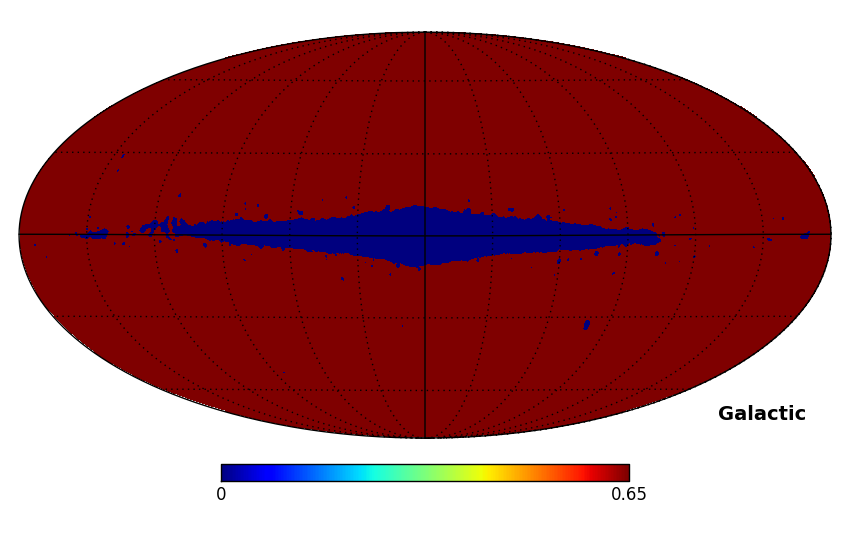
\includegraphics[width=\columnwidth,clip,trim=0 1in 0 0]{prod_mask}
  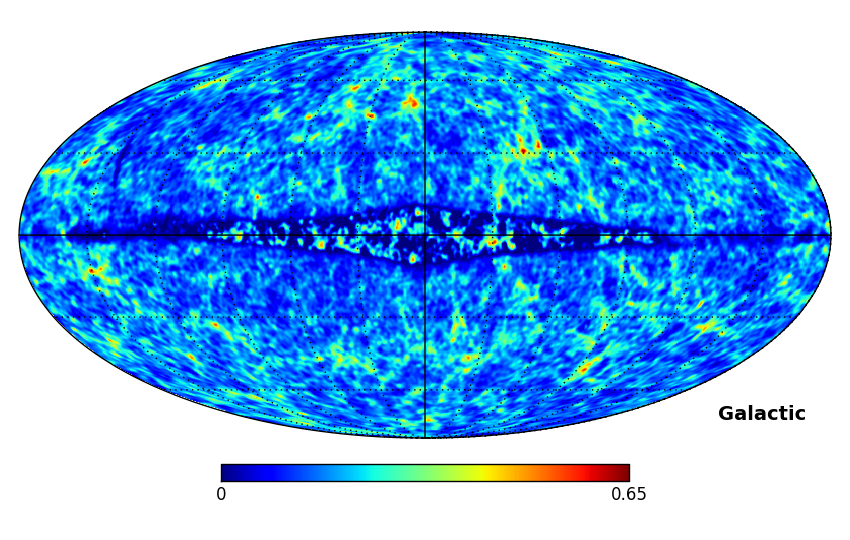
\includegraphics[width=\columnwidth]{infilled_prod_mask}
  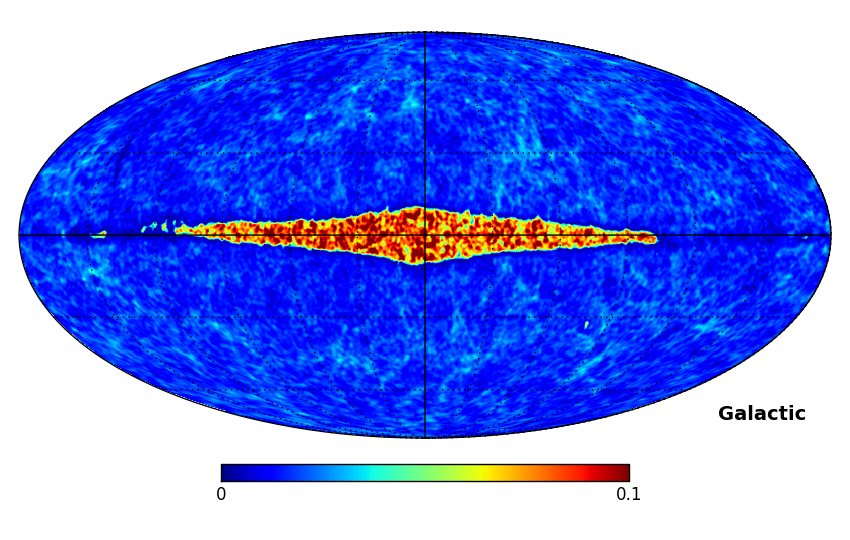
\includegraphics[width=\columnwidth]{sigma_prod_mask}
  \caption{Upper: the mask used for the infilling procedure obtained
    by determining the regions where the galaxy density is less than
    one tenth of the mean or the star denisty lies above a given
    threshold (see text for details).  Middle: the infilled galaxy
    distribution. Lower: The standard deviation of the infilled map
    obtained by bootstrapping the galaxy catalogue.}
  \label{fig:infilling}
\end{figure}

\section{Results}

To assess the performance of these techinques we will focus on optical
follow-up where we do not wish to observe through the zone of
avoidance.  We will use the Bayesian probability region calculated by
the BAYESTAR algorithm \citep{2015arXiv150803634S} from
\citet{2014ApJ...795..105S} for a LIGO-only detection, that is, before
Virgo is operational.  For simplicity we focus on fields of view that
correspond to a particular valid value of \texttt{NSIDE} for the
HEALPix map.  In particular we examine a 13-square-degree field of
view ($\mathtt{NSIDE}=32$) similar to that of LSST, 3-square-degree
($\mathtt{NSIDE}=64$), 0.8 and 0.2-square-degree fields of view.  We
quantify the performance in two ways: the time to create the optimized
observing plan is typically 1-3 seconds and the decrease in the number
of fields required to reach a given cumulative probability.  The time
to create the observing plan is typically less than the time to point
the telescope and begin observations, so the strategy would be to
point the telescope to the peak of the raw probability region and
calculate the observing plan during the slew.

Fig.~\ref{fig:bayestar} depicts the results for the different sizes of
fields and the possibility of using an raw (unsmoothed) and smoothed
galaxy map.  The upper panel gives the performance with a galaxy map
restricted to the redshift range $0.03<z<0.04$.  Here the improvement
in the number of fields to observe is most dramatic.  Let's start with
the lowest triplet of curves that correspond to the largest field of
view.  Here the improvement is of using a galaxy map is modest, the
number of fields to achieve a given cumulative probability decreases
by about 20\%.  This is because most 13-square-degree regions of the
sky contain a nearby galaxy. Furthermore, with such a large field of
view using a smoothed galaxy map does not affect the results
significantly.  On the other hand, if one uses the alternative metric
of what is the probabilty of that the source lies within the first
field, the use of a galaxy map increases this probability from about
6.5\% to 9.2\%.

If we now examine the most modest field of view, the 0.2 square-degree
field, we can see a more dramatic advantage of using the galaxy map.
If one uses the raw galaxy map in which each observed field must
contain at least one galaxy, it requires 57 fields (or about 12 square
degrees) to reach half of the cumulative probability.  To reach the
same cumulative probability requires 186 fields (about 40 square
degrees) if one uses the smoothed map and 308 fields (about 65 square
degrees) without a galaxy map.  For such a small field of view the
effectiveness of the galaxy map is dramatic.  Furthermore, the chance
of the source being in the first observed field increases from 0.26\%
to 2.3\% with the unsmoothed map.  Understandably for the
intermediate-sized fields of view the improvement is intermediate
between that achieved for the LSST field of view and for the modest one.

If the redshift estimate for the source is somewhat less accurate
perhaps $0.01<z<0.05$, the gains to be had by using a galaxy map are
more modest as depicted in the lower panel of Fig.~\ref{fig:bayestar}.
For the 13 square-degree field of view, the improvement is especially
modest; with the galaxy map eight fields are required to reach the
fifty percent mark and without the map nine fields are required.  For
the smallest field of view, the galaxy map reduces the number of
fields required to reach the fifty-percent mark from 308 to 141, a
55\% reduction.  With the more accurate redshift estimate the
reduction was over 80\%.  The probability of the source lying in the
first field increases from 0.26\% to 0.52\%.  This stresses the
importance of having distance estimates as early as possible in the
data analysis following a burst.
\begin{figure}
  \includegraphics[width=\columnwidth,clip,trim=0 1.35cm 0
    0]{T125738_bayestar_2MPZgz_003_004.pdf}
  \includegraphics[width=\columnwidth,clip,trim=0 0 0
    0.15cm]{T125738_bayestar_2MPZgz_001_005.pdf}
  \caption{The number of fields required to cover the given fraction
    of the probablity region for a simulated LIGO detection (red
    curves without the galaxy map, green curves with a smoothed
    galaxy, blue curves with a raw galaxy map).  The upper solid
    curves use a healpix map with about 200,000 cells, the dashed
    curves have about 50,000 cells, the dotted curves have about
    12,000 cells and lower solid curves have about 3,000 cells,
    corresponding 0.2, 0.8, 3.2 and 13 square-degree fields of
    view. The redshift range of the galaxy map in the upper panel is
    $0.03<z<0.04$ and $0.01<z<0.05$ in the lowel panel.}
  \label{fig:bayestar}
\end{figure}

\section{Conclusions}

The discovery of gravitational waves binary black hole highlights the
need for rapid three-dimensional localization of gravitational-wave
events to understand the astrophysical nature of these sources.
Although the Fermi GBM did see hints of gamma rays coincident with the
gravitational wave event in time \citep{2016arXiv160203920C}, other
efforts at finding an electromagnetic counterpart were apparently in
vain
\citep[e.g][]{2016arXiv160204198S,2016arXiv160204156S,2016arXiv160204488F},
possibly due to the rapid decay of the electromagnetic radiation from
the binary black-hole merger.  Only the GBM experiment though had
observations coincident in time with the event.  The Fermi LAT managed
to observe the entire probability region within 70 minutes of the
event, so the timescale for rapid follow-up of these events is minutes
rather than hours.  The algoriths presented in this paper offer a
technique to maximize the potential for discovery with a very modest
computation of the fields to observe first and which order.  The key
is to calculate the likely regions of sky to observed before the burst
in the form of a HEALPix map, so at the burst one can rapidly
construct the observing plan.

The information that one puts into the map, of course, will depend on
the nature of the gravitational-wave event ({\em e.g.} its distances,
the masses and composition of the components, {\em etc.}).  Here we
have simply used the surface density of nearby galaxies for the
$P(\mathrm{position})$ map.  However, one can do much better by using
the predicted rates of the various types of events and the types of
galaxies that one expects to find them in.  For example,
\citet{2016arXiv160204531B} argue that an event like GW150914 resulted
from a binary black hole whose progenitor stars formed around a
redshift of 3 (70\% likely) or around a redshift of 0.2 (30\%).  This
information informed by stellar population synthesis could be used to
develop a better guess for the galaxy map by increase the weight of
galaxies whose stars were born during these epochs.
\citet{2015ApJ...806..263D} argue that the coalesce of black-hole
binaries like GW150914 will dominate the detection rates, and
furthermore, most of these binaries form in low-metallicity galaxies
at about 1~Gyr after the Big Bang.  Knowing in which local galaxies
these systems typically end up would greatly improve the follow-up
strategy.  Are we interested in looking at systems that are still low
metallicity with star formation long ago like dwarf spheroidals?  Or
do we expect these systems to have been incorporated in larger galaxies
subsequently and are these larger galaxies typically spirals or
ellipticals today?

The dawn of gravitational wave astronomy is upon us.  To realize its
full potential we can used all of our prior knowledge of the expected
rates of these event in the context of the hierarchical formation of
galaxies to determine where to look for the electromagnetic signal
that hopefully accompanies these events.


The software used in this paper is available at
\url{http://ubc-astrophysics.github.io}.  We used the VizieR Service,
the NASA ADS service, the SuperCOSMOS Science Archive, the NASA/IPAC
Infrared Science Archive, the HEALPy libraries and arXiv.org. This work
was supported by the Natural Sciences and Engineering Research Council
of Canada, the Canadian Foundation for Innovation, the British
Columbia Knowledge Development Fund and the Bertha and Louis Weinstein
Research Fund at the University of British Columbia.


\bibliography{obsplan}
\bibliographystyle{apj}


\label{lastpage}
\end{document}
